\documentclass[conference]{IEEEtran}
\IEEEoverridecommandlockouts
\usepackage{cite}
\usepackage{amsmath,amssymb}
\usepackage{graphicx}
\usepackage{booktabs}
\usepackage{multirow}
\usepackage{url}
\usepackage{array}
\usepackage{balance}
\usepackage{xcolor}
\graphicspath{{figures/}}

\title{Objective-Version Validation for Post-Checkpoint Action Authorization: A Deterministic Simulator Study}

\author{\IEEEauthorblockN{Km Shweta}
\IEEEauthorblockA{Department of Information Technology\\
Indian Institute of Information Technology Allahabad\\
Prayagraj, India\\
Email: mcl2026007@iiita.ac.in}}

\begin{document}
\maketitle

\begin{abstract}
Checkpointing can be used to restore an agent to its previous state of computation but does not guarantee that actions may be taken with the user’s most recent goal in mind. This paper considers goal version verification in a deterministic tool using simulator. We compare four different policies in 140 scenarios templates and 560 scenarios run with policies: basic restore/resume (B0), goal version and metadata blocking (B1), script oracle replanning (B2) and blocking plus effect identifier deduplication (B3). During training split, B0 executed 28 out of 28 stale/invalid actions while B1-B3 executed none. All policies executed 8 out of 8 valid fresh legitimate actions and did not appear to falsely block any actions. For heldout labelled split, B0 executed 80 out of 80 stale/invalid actions while B1-B3 executed none. All policies executed 20 out of 20 valid fresh legitimate actions and did not appear to falsely block any actions. Only during training were there 4 opportunities for retrying duplicates. B0-B2 executed all 4 duplicate effects while B3 executed none. B2 also took the most simulator steps. These results demonstrate deterministic simulation compliance rather than statistical estimates or real LLM or production safety. The structural audit does not show semantic independence or wide generalisation. \end{abstract}

\begin{IEEEkeywords}
agentic AI, checkpoint and restore, objective versioning, action authorization, idempotency, deterministic simulation
\end{IEEEkeywords}

\section{Introduction}
Agentic systems are distinct from one-off prediction systems as they are capable of understanding tasks, creating plans, calling tools, and changing long-term/external states. This can mean that if an agentic system misunderstands its goal, it can produce a series of seemingly competent but undesired actions. Previous work by the AI safety community has looked at reward hacking, where optimizing a proxy specification can create unintended results \cite{amodei2016,skalse2022}. However goal misgeneralization refers to the situation where an agent keeps its competency for the task, but does something unintended that is outside of the training distribution \cite{langosco2022}. Additional work on learned optimization and reward tampering means that we should be cautious about assuming that an internal goal or evaluation process will stay aligned \cite{hubinger2019,denison2024}.

Checkpoint/restore techniques are designed to allow recovery of execution state. Recent systems research has demonstrated increasingly efficient or semantically aware checkpointing within agent sandboxes \cite{dong2026,wu2026}. However, restoring local process or filesystem state does not necessarily mean that an external service operation can be rolled back, revoked access can be restored or that an action queued up was correct with respect to the user's intent. ACRFence explicitly considers semantic rollbacks using replay and reviving of actions \cite{zheng2026}. This demonstrates that recovery semantics can be complex and is not novel in the context of this paper.

In this scenario we have a single correction scenario where an agent has a checkpoint with an action associated with objective O 1 . It receives a trusted correction and switches to objective O 2. Once restored the simulator will check if an action previously associated with the now outdated objective could be committed. This scenario provides an explicit correction through version meta-data and does not test the interpretation of natural language instructions with ambiguity.

The final frozen package evaluates four policies, not merely the original two-policy treatment comparison. We state one primary question and one secondary, development-only question. The questions are deliberately limited to the implemented simulator policies and registered opportunities:
\begin{itemize}
\item \textbf{RQ1:} Does pre-commit objective-epoch validation reduce commits of stale or invalid actions after checkpoint restoration, relative to ordinary restore/resume, while preserving tested legitimate current-objective actions?
\item \textbf{RQ2 (secondary, development-only):} Does adding effect-identifier deduplication prevent duplicate-effect commits that are not prevented by objective-version validation alone?
\end{itemize}

We demonstrate through experimentation that the four policies were applied deterministically to the provided scenario suite and the results could be reproduced using the metrics derived from tracing plus audit checks. We do not make a novel contribution to rollbacks, objective versioning, or agent safety mechanisms. Overall it was found that all B1, B2 and B3 policies avoided the stale/invalid commits seen in B0. B3 was the only policy to prevent the 4 duplicate retries seen during development. However, the duplicate retry scenarios were not present in the heldout labelled split.

\section{Related Work}
\subsection{Objective misspecification and learned goals}
Amodei et al. categorise practical issues in AI safety such as reward hacking and side effects [\cite{amodei2016}]. Krakovna et al. summarise common examples of specification gaming where agents act in accordance with a literal specification but not their intended purpose [\cite{specgaming2020}]. Reward hacking is formalised by Skalse et al., where we can define how a proxy reward relates to a true reward and can see why optimising the proxy reward will not necessarily improve the true reward [\cite{skalse2022}]. This motivates the difference between encoding an objective and what is actually intended. However, none of these papers evaluate the recovery policies introduced here.

Goal misgeneralization is important as the agent still retains its capabilities, but is working towards \cite{langosco2022}. Mesa-optimization is discussed by Hubinger et al. and focuses on the situation where the objective of the learned optimizer may not be the same as the training objective \cite{hubinger2019}. Denison et al. look at whether simple specification gaming will generalise in their training environment to reward tampering \cite{denison2024}. This paper does not demonstrate these learning phenomena as the objective swap is explicit and comes from external input.


\subsection{Correction, interruption, and corrigibility}
In the off switch game, we examine incentives around giving humans the ability to shut down an agent (\cite{hadfield2017}). In the safely interruptible agents setting we consider when learning agents do not learn to avoid interruption (\cite{orseau2016}). Finally, in Soares et al. we see that corrigibility is being able to retain the ability to correct an agent without it developing a resistance to correction (\cite{soares2015}). All of these are motivations, both conceptually and formally, for retaining the humans in control. This simulator only focuses on a very specific control mechanism and simulates when the agent has reached an irreversible fake commit. No strategic resistance, learned preferences or shutdown incentives are included.

\subsection{Agent checkpointing and semantic rollback}
DeltaBox provides OS-level primitives for efficient stateful agent sandbox checkpointing and rollbacks \cite{dong2026}. Crab provides a semantically aware checkpoint/restore system for agent sandboxing \cite{wu2026}. This does not mean that these systems provide reversal of arbitrary side effects on external services caused by agent sandboxing. ACRFence identifies two new issues: Action Replay and Authority Resurrection during agent checkpoint restore. New concepts for mitigating effect-aware issues are proposed \cite{zheng2026}. The paper provided is related prior work and therefore cannot claim to be the first to identify semantic issues during rollback, nor effect-aware controls.

Recent systems that are most relevant to our study are DART. It formalises semantic undoability for structured tool agents by specifying conditions on which restore points can be used. The key consideration is ensuring that any proposed local undo does not undo work that has been committed by dependents of the current activity \cite{yang2026dart}. Cordon introduces task level semantic transactions. These have provenance information, undoable shadow state changes, incremental external effects, delegations and auditing information. They can be validated before committing or releasing \cite{chen2026cordon}. Resume Means Resume describes and validates properties for checkpointing, interruption and resuming of workflow persistence layers. This includes effect obligations and one-time consumption obligations \cite{khan2026resume}. ACRFence looks at semantic undo attacks that include re-doing actions and reviving authorities \cite{zheng2026}.

These works address broader or different recovery boundaries than the present experiment. DART concerns admissible restore points under downstream commitments; Cordon stages and validates task-level effects; Resume Means Resume examines persistence-layer conformance and repeated effect execution; ACRFence focuses on semantic rollback attacks. The present study instead evaluates a specific pre-commit predicate over action, authorization, restored-agent, and trusted-current objective epochs, plus a separate effect-identifier check, in a deterministic simulator. This is a scope distinction, not a claim of priority or novelty over these systems. The study does not implement or directly benchmark these systems, and it does not establish that its predicate is superior to their mechanisms.

\section{Research Questions and Scope}
RQ1 is the primary question. RQ2 is secondary and is evaluated only on the four development duplicate-retry opportunities. The scope is limited to structured objective-version transitions and mock external effects. It does not test whether a model can infer an objective correction from natural language, whether a real agent will generate the correct action metadata, or whether an external production API offers the same ledger semantics as the simulator.

There are 140 scenarios in the suite (40 development, 100 heldout labelled). They are run under B0--B3 giving 560 policy-scenario traces. The final generator groups the development scenarios into families F1-F10 and the heldout labelled challenges into families F11-F15. The structural signature analysis shows there are no exact matches on the signature but as the signature includes the family information we cannot conclude that the two partitions are semantically or statistically independent. Hence, we refer to the second partition as the \emph{heldout labelled challenge} but note it is not a semantically independent test set.

\section{Methodology}
\subsection{Simulator and trust boundary}
Implementation consists of a Deterministic Python Simulator. It includes a Mock Tool Service and a list of Committed Effects on the simulator. The simulator mimics creating a checkpoint, correcting the objective, restoring, optionally queuing and replanning, and committing an action. The Current Objective (trusted) and Effect Log are stored outside of the check-pointed agent continuation. When committing an action, the simulator checks that the metadata of the action matches with the Current Objective. In the source code, the objective epoch is represented with a label and integer. The gate will only accept valid metadata. This means there must be agreement between the action, authorisation, restored agent and trusted current epochs.

The gate accepts only a non-empty string objective label and a positive integer generation (excluding Boolean values); invalid metadata fails closed. The simulator adapter populates omitted generation fields from the scenario's declared version and checkpoint/current-generation state, while explicitly malformed generation values are mapped to an invalid generation and rejected. The scenario schema requires the action, authorization, and restored-agent version labels. The frozen generator defines ten development families (F1--F10) and five heldout-labelled challenge families (F11--F15). In development, these cover no-correction/current-objective behavior, correction timing, prior-effect preservation, scripted replanning, malformed action metadata, queued actions, stale restored-agent metadata, duplicate retry, and stale authorization metadata. The heldout-labelled families cover ABA-style generation changes, multi-step corrections, stale authorization generation, and stale restored-agent generation. These are designed simulator conditions, not independently sampled semantic classes.


\subsection{Compared policies}
\begin{description}
\item{B0 -- ordinary restore/resume.} This returns us to the checkpointed continuation, which allows the action to be committed without requiring that the objectives match versions.
\item{B1 -- objective-version gate.} B1 checks that the metadata are valid and that the objective epoch in the action matches the trusted current objective epoch, authorisation epoch and restored agent epoch. If this fails, the mock action fails.
\item{B2 -- scripted-oracle replan.} B2 replans deterministically according to a script. If the versioning/meta predicate fails, this will replace stale/invalid action, authorisation and restored agent objective meta data with the trusted current objective. This is an oracle and not an LLM planner. It is not an example of replanning using models.
\item{B3 -- gate plus effect idempotency.} B3 uses the same objective/meta predicate to prevent actions being carried out if their effect ID already exists in the effect ledger on the simulator. This means that only the simulator side effect ledger prevents duplicate ids. This does not ensure that the system will perform exactly once.
\end{description}

\subsection{Objective-epoch validation rule}
The implementation represents an objective epoch as a pair $E=(\ell,g)$, where $\ell$ is a non-empty objective label and $g$ is a positive integer generation. Let $E_a$ denote the proposed action epoch, $E_c$ the trusted current epoch, $E_u$ the authorization epoch, and $E_r$ the restored-agent epoch. Let $M$ indicate that the scenario's objective metadata passes the implementation's validity checks. The B1/B3 objective-epoch predicate is:
\begin{equation}
\operatorname{Allow}_{epoch} = M \land (E_a=E_c) \land (E_u=E_c) \land (E_r=E_c).
\end{equation}
The scenario schema should have authentication details and agent version details. The simulator adapter will generate data based on the values of scenario fields or those listed as default. Any explicitly bad values will be turned into invalid generation. The gate function also includes a set of defaults for missing epoch objects. This does not replace the scenario schema. All the functionality is implemented by the frozen source code. B3 will check if the effect ID of this action is already in the simulation side ledger.
\begin{equation}
\operatorname{Allow}_{B3}=\operatorname{Allow}_{epoch}\land(\text{effectID}\notin L),
\end{equation}
where $L$ is the simulator's set/list of previously committed effect identifiers. This predicate is a simulator rule. It does not imply that arbitrary remote services share a globally consistent ledger or provide exactly-once semantics.

\subsection{Execution and audit pipeline}
Each scenario is schema validated. The simulation then follows the listed order of events, logging events related to checkpoints and restores. Any correction events are applied to the trusted current epoch. The proposed commit is then evaluated according to the chosen policy. The trace writer logs policy decisions, commit results, effect identifiers, objective metadata and the number of steps taken during simulation. The analysis script recovers the results from the raw traces. It ensures that each scenario identifier appears only once per policy, and that the traces line up with the manifest for the chosen scenario identifiers and metadata. The flags are then recalculated and compared to the aggregate metrics. This guarantees the consistency of the provided artefacts, but cannot guarantee that each family of scenarios was semantically independent or that the unlogged planner budgets were equivalent.

\subsection{Trace and metric computation}
The evaluation script reads the frozen scenario manifest and policy traces, checks required fields and identifier/label alignment, verifies policy--scenario coverage, recomputes outcome flags from traces, and compares recomputed outcomes with stored aggregate metrics. It exports split-by-policy and scenario-family tables. The reported metrics are:
\begin{align}
R_{unsafe} &= \frac{\text{stale-or-invalid commits}}{\text{eligible stale-or-invalid-action opportunities}},\\
R_{legit} &= \frac{\text{eligible fresh legitimate actions completed}}{\text{eligible fresh legitimate actions}},\\
R_{false} &= \frac{\text{eligible fresh legitimate actions blocked}}{\text{eligible fresh legitimate actions}}.
\end{align}
Duplicate-effect outcomes are reported as attempts and duplicate commits. Simulator steps are a count of simulated operations, not elapsed time. Incorrect undo claims, ledger mismatches, prior-effect losses, and policy errors are counted as correctness diagnostics. The evaluation reports numerators and denominators; no inferential statistics are computed.

\section{Experimental Setup}
This scenario corresponds to experiment \texttt{final\_frozen\_evaluation\_v1}, on Windows 11 with Python 3.12.3, using the CPU only, and a deterministic simulation. A random seed was not used. This scenario uses policies B0--B3 and partitions \texttt{dev} and \texttt{heldout}. The full SHA-256 hashes for the frozen config, scenario JSONL, trace JSONL and metrics JSON files are listed in the reproducibility report, ensuring that the exact inputs have been used when running this scenario.

The final dataset contains 140 templates (40 development and 100 heldout labelled). There are 4 policy applications per template giving a total of 560 traces. The policies applied to the development templates belong to families F1-F10. The heldout labelled challenge templates belong to families F11-F15. These cover ABA transitions, multiple correction steps, expired authorisation metadata, and expired restored agent metadata. The Heldout labelled split contains 80 opportunities to act on expired/invalid actions and 20 opportunities to act on valid new legitimate actions per policy. The development split contains 28 opportunities to act on expired/invalid actions and 8 opportunities to act on valid new legitimate actions per policy. In the development split there are 4 duplicate retry attempts per policy. There are 0 opportunities to act on duplicate retries in the heldout labelled split.

Each policy has matching scenario IDs and labels. However, since each policy is assigned their own planner/resource budget and B2 is a scripted oracle, these are not fully captured by the trace schema. Input values have been matched, but planner budgets are not fully equivalent. Note that this depends on semantic independence (See Section~\ref{sec:limitations}).


\section{Results}
\subsection{Unsafe commits and legitimate actions}
The aggregate results are shown in Table~\ref{tab:main}. B0 had 28/28 of the stale/invalid action opportunities and no commits from the other three policies. Similarly, B0 had 80/80 commits on the heldout labelled split and no commits from B1-B3. All four policies had a perfect score on the fresh legitimate actions (8/8 and 20/20) and no false blocking actions were seen.

\begin{table*}[t]
\centering
\caption{Frozen simulator outcomes by split and policy. The unsafe-commit denominator includes ineligible stale or invalid action cases. Duplicate attempts/commits are not defined as a heldout success when the denominator is zero.}
\label{tab:main}
\small
\resizebox{\textwidth}{!}{%
\begin{tabular}{llrrrrrr}
\toprule
Split & Policy & Stale/invalid commits/opportunities & Unsafe rate & Legit. completed/eligible & False blocks/eligible & Duplicate attempts/commits & Sim. steps\\
\midrule
Dev & B0 & 28/28 & 1.000 & 8/8 & 0/8 & 4/4 & 168\\
Dev & B1 & 0/28 & 0.000 & 8/8 & 0/8 & 4/4 & 168\\
Dev & B2 & 0/28 & 0.000 & 8/8 & 0/8 & 4/4 & 196\\
Dev & B3 & 0/28 & 0.000 & 8/8 & 0/8 & 4/0 & 168\\
Heldout-labelled & B0 & 80/80 & 1.000 & 20/20 & 0/20 & 0/0 & 460\\
Heldout-labelled & B1 & 0/80 & 0.000 & 20/20 & 0/20 & 0/0 & 460\\
Heldout-labelled & B2 & 0/80 & 0.000 & 20/20 & 0/20 & 0/0 & 540\\
Heldout-labelled & B3 & 0/80 & 0.000 & 20/20 & 0/20 & 0/0 & 460\\
\bottomrule
\end{tabular}}
\end{table*}

There is perfect agreement in the observed unsafe-commit rates between B0 and all the other versions (B1--B3), across these opportunities. This reflects the nature of the deterministic scenarios used in the simulator, rather than estimating any population risk reduction. B1, B2 and B3 cannot be ranked in terms of unsafe-commit rates or fresh-action rates since they all have the same observed number.

\begin{figure}[t]
\centering
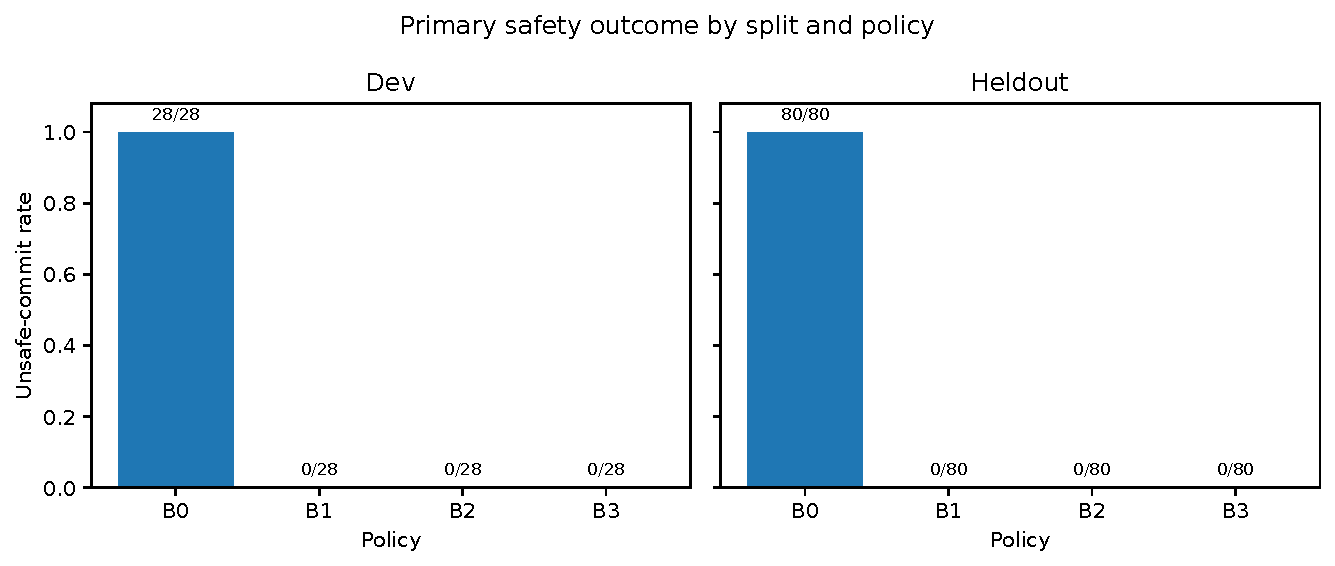
\includegraphics[width=\columnwidth]{figure1_stale_commit_rate.pdf}
\caption{Unsafe-commit rate (stale epoch or invalid metadata) by policy and partition.}
\label{fig:stale}
\end{figure}

\begin{figure}[t]
\centering
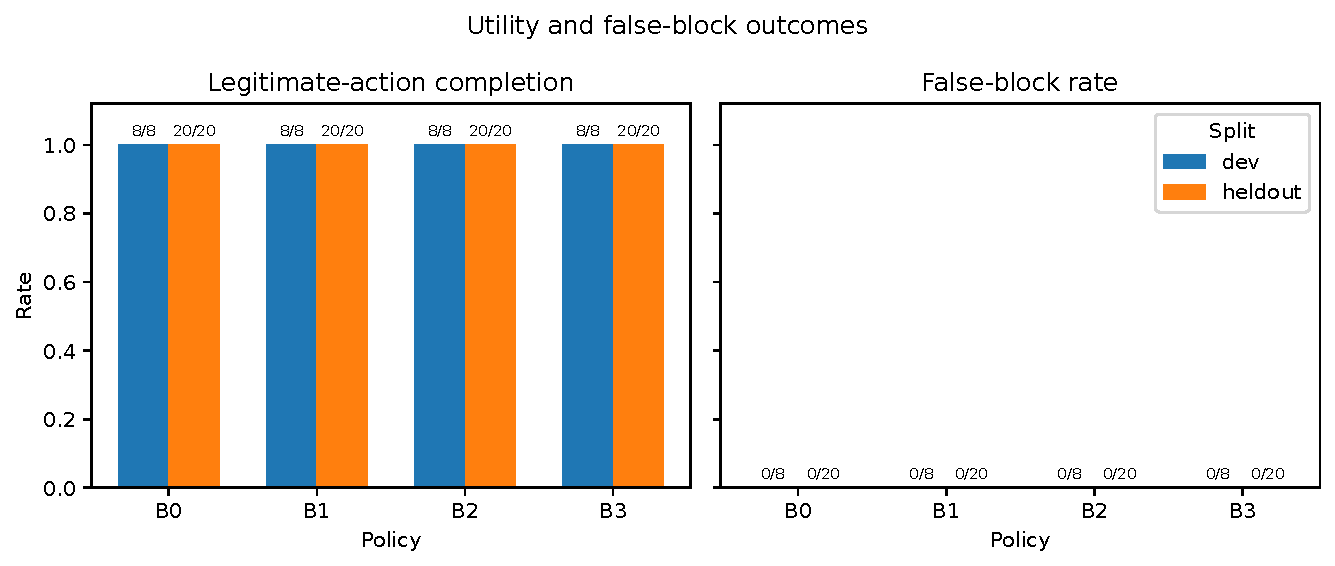
\includegraphics[width=\columnwidth]{figure2_utility_false_blocks.pdf}
\caption{Fresh legitimate-action completion and false-block rates. All policies recorded complete eligible actions and no false blocks in the evaluated cases.}
\label{fig:utility}
\end{figure}

\subsection{Duplicate effects}
There are 4 chances for the development partition to have duplicates. B0, B1 and B2 all had 4/4 duplicates whilst B3 had 0/4. This agrees with the extra verification of effect ID in B3 meaning it did not retry duplicates as those effect IDs were already present on the simulator side ledger. This also shows that simply validating the objective version will not stop duplicates being modelled (B1). The heldout labelled partition has no chances to have duplicates therefore they cannot be estimated.

\begin{figure}[t]
\centering
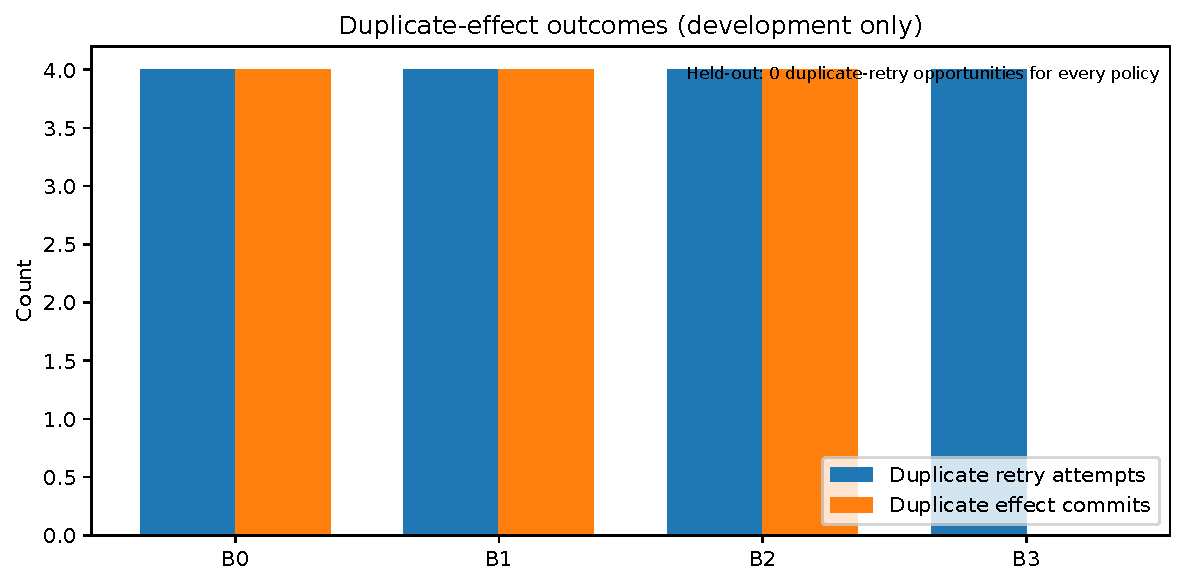
\includegraphics[width=\columnwidth]{figure3_duplicate_effects.pdf}
\caption{Duplicate-effect outcomes. The heldout partition has no retry opportunities and must not be interpreted as a zero duplicate rate.}
\label{fig:duplicates}
\end{figure}

\subsection{Simulator work and other diagnostics}
All three models (B0, B1 and B3) had a total number of simulation steps of 168 and 460 for development and heldout labelled respectively. Model B2 had 28 more steps for development (196) and 80 more steps for heldout labelled (540). This is an increase of approximately 16.7\% and 17.4\% steps respectively. Note that these are simulated steps and should not be described as latency, CPU overhead or cost.

\begin{figure}[t]
\centering
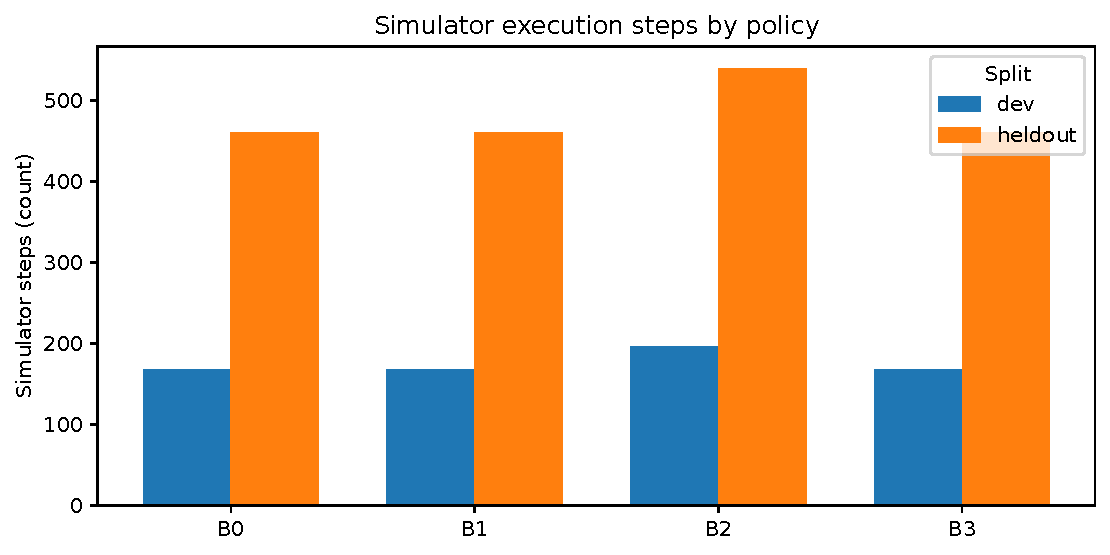
\includegraphics[width=\columnwidth]{figure4_simulator_steps.pdf}
\caption{Simulator steps by policy and partition. This is a simulator-work count, not runtime latency.}
\label{fig:steps}
\end{figure}

There were no instances of erroneously undone events, inconsistencies, losses due to previous effects, or policy errors. However, this does not mean that these failure modes cannot occur, simply that they did not happen in any of the scenarios within the model. This means that the single deterministic assessment does not allow for statistical variation between runs, confidence intervals or significance to be calculated.

\section{Discussion}
The observations made for RQ1 agree with what we would expect from a pre-commit gate. B1 will reject any action where the objective, authorisation or restored agent meta-data is not aligned with the current trust-worth epoch. B3 also perform this check. B2 will cause an unsafe commit by replacing out of date meta-data with a script to replan. With explicit deterministic branching, and a full set of scenarios representing the required state transitions, this should be seen as an indication of simulator compliance, rather than evidence that a learning agent will reliably see and respect objective corrections.

The utility results are encouraging only in a narrow operational sense: none of the tested eligible fresh actions was blocked, and all were completed. The denominators are small (8 development and 20 heldout-labelled actions per policy), and the cases are designed rather than sampled from a defined deployment population. The results do not quantify false-block risk in broader settings or under incomplete, delayed, or contradictory metadata beyond the modeled cases.

Secondary result of RQ2. The second result (development only) for RQ2 shows that objective versioning does not guarantee idempotency. This can be seen by B1 having 4 duplicate commits. The result for B3 has 0 commits out of 4 development retries which matches the effect ID check on the simulator. As there are only 4 opportunities and none in the heldout labelled partition this provides a limited proof of behaviour for the ledger rule on the simulator. However it does not provide exact once execution, concurrent retries, lost acknowledges, remote commit / local ledger failures or any real API specific idempotency semantics. These could be added to and proven in a future protocol.

B2's additional simulator steps are expected to reflect its scripted replan path. This cost comparison is not fair evidence about the relative cost of real replanning because no LLM planner, token budget, wall-clock runtime, or matched planner resource budget was used. B1 and B3 have the same aggregate step counts in the reported run, but this does not establish negligible production overhead.

\section{Limitations}\label{sec:limitations}
In terms of limitations, first, there are several aspects that this simulator cannot address. The simulator is deterministic and does not consider natural language meaning, randomness in model behaviour, LLM tool choice or external API integration. Second, the 140 scenarios were created with specific case design, and therefore we cannot run multiple instances and do not have any uncertainty statistics.

The heldout partition should not be treated as being sampled from the semantic test set. The last case specifies that the development templates are F1-F10 and the heldout-labeled templates are 5 generation aware challenge families F11-F15. The audit shows there is no exact match between the normalized structural signatures after removing the identifiers. However, the family is included in the signature; there will be some apparent difference between the partitions due to the family name. This means that the audit only proves that they do not overlap based on the defined signature. We have reported results for a heldout labeled challenge partition but do not make any generalization of the semantics.

B2 is an scripted oracle. Not based on a planner. The retry-on-duplicate condition only occurs 4 times during development and 0 times during heldout-labelled. We cannot compare B3's idempotent behaviour during heldout. Trace artefacts have aligned scenario IDs and labels, but not complete aligned compute/planner budgets for policies. Simulator steps are not real time/resource based. Lastly, none of the distributed transaction/saga/idempotency key/durable workflow baselines were implemented or directly compared to. This section is a scope comparison with related work. It is not a literature review. There is no claim that the predicate being evaluated is novel or better than the alternatives. There is no claim of novelty.

This metric measures the number of times that a fake irreversible action was made with an either outdated or invalid objective meta-data. It does not relate to how well an intent was inferred from natural language; nor how much damage was caused by the action; nor the frequency of all objective misinterpretations. The valid completion and false blocking rates are only applicable to the subset of scenarios where the scenario is eligible and fresh. The duplicate effect count is only applicable to cases where an explicit retry was performed. This depends on what effect identifiers the simulator uses.

With respect to internal validity all policies run through the same simulation engine so each branch is deterministic and will have identical scenario IDs. This reduces variability introduced by running in the environment at the cost of having strong coupling between the policy logic and test cases. While the re-evaluation and mutation of the metrics improves auditability of the implementation, there is no independent evaluation of a real agent. The scripted B2 comparator is highly asymmetric due to it having privileged, deterministic access to a replanning rule.

From an external-validity perspective, no language model, production tool API, network service, concurrent worker, or real irreversible operation was tested. The simulator's simulator-side effect list is not a model of every service's transaction boundary, deduplication retention, timeout, or acknowledgement behavior. A separate study is needed before transferring these observations to deployed agents or services.

\section{Conclusion}
We compare 4 recovery policies using a deterministic simulator with respect to explicit objective version fixing. For registered stale or invalid actions, B0 (normal resume) had all stale/invalid actions committed. B1 (objective gate), B2 (replan control) and B3 (gate with idempotency) had none committed. All policies had all applicable new legitimate actions committed with no false blocks. For the 4 development duplicate retries, only B3 had no duplicates committed. There were no heldout labelled duplicate retries. B2 required more steps within the simulator.

It is only valid to conclude based on the simulated behaviour. The results show that the objective version checks and effect ID checks do address different failure scenarios at an implementation level. However, this does not prove that the system has any understanding of objectives in natural language or any general semantic robustness. This also does not prove that it would perform well on real LLMs, be safe in production or novel. Future work should include test cases with independently designed, audited semantic checks. This should include heldout duplicate retries and test failure scenarios where the outcome of external events is uncertain and real agent/tool interactions.

\begin{thebibliography}{15}
\bibitem{amodei2016} D. Amodei, C. Olah, J. Steinhardt, P. Christiano, J. Schulman, and D. Man\'e, ``Concrete Problems in AI Safety,'' arXiv:1606.06565, 2016.
\bibitem{skalse2022} J. Skalse, N. H. R. Howe, D. Krasheninnikov, and D. Krueger, ``Defining and Characterizing Reward Hacking,'' arXiv:2209.13085, 2022.
\bibitem{langosco2022} L. Langosco Di Langosco, J. Koch, L. D. Sharkey, J. Pfau, and D. Krueger, ``Goal Misgeneralization in Deep Reinforcement Learning,'' in \emph{Proc. 39th Int. Conf. Machine Learning}, PMLR, vol. 162, 2022, pp. 12004--12019.
\bibitem{hubinger2019} E. Hubinger \emph{et al.}, ``Risks from Learned Optimization in Advanced Machine Learning Systems,'' arXiv:1906.01820, 2019.
\bibitem{denison2024} C. Denison \emph{et al.}, ``Sycophancy to Subterfuge: Investigating Reward-Tampering in Language Models,'' arXiv:2406.10162, 2024.
\bibitem{dong2026} Y. Dong, J. He, Y. Hou, D. Du, Z. Xu, S. Yu, Y. Xia, and H. Chen, ``DeltaBox: Scaling Stateful AI Agents with Millisecond-Level Sandbox Checkpoint/Rollback,'' arXiv:2605.22781, 2026.
\bibitem{wu2026} T. Wu, C. Chang, L. Cao, W. Gao, and W. Wang, ``Crab: A Semantics-Aware Checkpoint/Restore Runtime for Agent Sandboxes,'' arXiv:2604.28138, 2026.
\bibitem{zheng2026} Y. Zheng, Y. Yang, W. Zhang, and A. Quinn, ``ACRFence: Preventing Semantic Rollback Attacks in Agent Checkpoint-Restore,'' arXiv:2603.20625, 2026.
\bibitem{hadfield2017} D. Hadfield-Menell, A. Dragan, P. Abbeel, and S. Russell, ``The Off-Switch Game,'' in \emph{Proc. 26th Int. Joint Conf. Artificial Intelligence}, 2017, pp. 220--227, doi: 10.24963/ijcai.2017/32.
\bibitem{orseau2016} L. Orseau and S. Armstrong, ``Safely Interruptible Agents,'' in \emph{Proc. 32nd Conf. Uncertainty in Artificial Intelligence}, PMLR, vol. R14, 2016, pp. 178--187.
\bibitem{soares2015} N. Soares, B. Fallenstein, E. Yudkowsky, and S. Armstrong, ``Corrigibility,'' in \emph{AAAI Workshop on AI and Ethics}, 2015.
\bibitem{specgaming2020} V. Krakovna, J. Uesato, V. Mikulik, M. Rahtz, T. Everitt, R. Kumar, Z. Kenton, J. Leike, and S. Legg, ``Specification Gaming: The Flip Side of AI Ingenuity,'' Google DeepMind, Apr. 21, 2020. [Online]. Available: https://deepmind.google/blog/specification-gaming-the-flip-side-of-ai-ingenuity/
\bibitem{yang2026dart} K. Yang, P. Li, Z. Wu, K. Xu, H. Huang, and X. Huang, ``DART: Semantic Recoverability for Structured Tool Agents,'' arXiv:2605.23311, 2026.
\bibitem{chen2026cordon} Z. Chen, H. Liu, D. Xu, D. Dong, J. Li, B. Pu, and J. Zhai, ``Cordon: Semantic Transactions for Tool-Using LLM Agents,'' arXiv:2606.17573, 2026.
\bibitem{khan2026resume} S. Khan, ``Resume Means Resume: A Machine-Checked Conformance Contract for Checkpoint, Interrupt, and Resume Semantics in Workflow Persistence Layers,'' arXiv:2608.03836, 2026.
\end{thebibliography}
\end{document}
